\chapter{Ondas --- Introdução}
\textsl{{\sffamily(Versão: \today)}}

\noindent
Neste capítulo, vamos considerar fenómenos óticos que não são descritos pelas
leis da ótica geométrica: a interferência, a difração e a polarização da luz.
A descrição e compreensão destes (e doutros) fenómenos é feita com base numa
teoria sobre a natureza da luz (coisa que até agora preferimos dispensar)
que, veremos, permite também deduzir as próprias leis da ótica geométrica. É,
pois, discutindo a natureza da luz que começamos este capítulo.

\section{Propagação corpuscular e ondulatória}
A luz é, claramente, \emph{algo} que se propaga. Mas o que é esse \emph{algo},
ao certo, e como é que se propaga?

Podemos classificar os processos de propagação em dois tipos principais. Nos
processos ditos \emph{corpusculares}, a entidade propagada de um ponto do espaço
para outro é transportada por partículas materiais (ou seja, em última análise,
por átomos) que percorrem a totalidade do percurso entre os dois pontos.
Exemplos deste tipo de propagação são as correntes oceânicas, o vento, as
correntes dos rios, as correntes de conveção, os deslizamentos de terras e
avalanches, etc. Nestes exemplos, verifica-se a propagação de energia (térmica
e/ou cinética), de momento linear, de momento angular, de relações de
causalidade\footnote{Por exemplo, a fratura na superfície de uma placa de neve
consolidada no alto da montanha provoca uma avalanche que soterra um grupo de
montanhistas mais abaixo na encosta: a causa (fractura) e o efeito (tragédia dos
montanhistas) não ocorrem no mesmo lugar; logo a relação de causa-efeito teve
que viajar entre os dois sítios, teve que se \emph{propagar}.}, sempre
acompanhadas do movimento macroscópico de matéria (e é este movimento de matéria
que transporta as outras entidades propagadas que referi).

Mas há também a possibilidade da propagação de quantidades físicas ou relações
causais não ser acompanhada de movimento macroscópico de matéria. Por exemplo,
quando uma pedra cai na superfície calma de um lago, são originadas ondas de
forma circular que se propagam até às margens do lago, transportando 
energia e momento linear. A propagação destas ondas entre o ponto onde
a pedra cai e a margem não é acompanhada por uma corrente superficial da água.
Cada pequena porção de água na superfície do lago apenas sofre uma oscilação
vertical quando a onda passa. Outro exemplo: o som que se propaga desde um
instrumento musical até aos nossos ouvidos. O instrumento anima as camadas de
ar que lhe estão próximas de um movimento de vibração microscópico e esse
movimento de vibração vai sendo comunicado entre porções de ar contíguas até
estar em vibração a camada de ar que está encostada à membrana do tímpano nos
nossos ouvidos. Neste processo, apenas se propagou o estado de vibração, não
foi necessário que as moléculas de ar viajassem desde o instrumento musical até
nós. Este tipo de propagação, em que não há movimento significativo de matéria,
ou ainda, por outras palavras, que não é acompanhado por um correspondente
transporte de massa, chama-se propagação \emph{ondulatória}.

Dada a maneira como acabámos de classificar os fenómenos de propagação, podemos
agora recolocar a pergunta com que começámos este capítulo: a luz é um
fenómeno corpuscular ou um fenómeno ondulatório? Isto é, a luz consiste num
chuveiro de pequenas partículas que viajam desde as fontes de luz até aos
objetos iluminados e destes até aos nossos olhos, ou trata-se antes de uma
perturbação do valor de alguma propriedade do espaço ou do estado de vibração de
algum meio material que percorre esse trajeto, sem que haja um correspondente
deslocamento de qualquer tipo de partícula?

As primeiras respostas dadas a esta pergunta foram fornecidas por Huygens, em
1678, e por Newton, em 1704. Enquanto que o primeiro acreditava na natureza
ondulatória da luz, o segundo considerava-a constituída por partículas.

Note-se
que ambos apresentaram argumentos sólidos a favor das hipóteses que defenderam:
\begin{itemize}
\item
    Huygens entendia que a luz devia ser um fenómeno ondulatório porque não eram
    observados sinais de colisões entre as partículas de luz de dois feixes que
    se cruzavam; logo, dizia, essas partículas não existiam e, portanto, a luz
    só podia ser um fenómeno ondulatório. Para além disso, a hipótese
    ondulatória permitia explicar os fenómenos da ótica geométrica mais
    simplesmente do que a hipótese corpuscular;
\item
    Newton, por seu turno, notava que a luz se propaga em linha recta, ao
    contrário das ondas do mar ou do som. Além disso, uma propagação
    ondulatória (que tem na base, pensava ele, uma vibração da matéria) não
    deveria ser possível na ausência de matéria. Ora, como a luz das estrelas
    chega até nós depos de atravessar o vazio interestelar, ela não poderia
    assim ser um fenómeno ondulatório.
\end{itemize}
A opinião de Newton prevaleceu durante cerca de cem anos, até que, em 1801,
Thomas Young e Augustin-Jean Fresnel mostraram através de experiências de
interferência que a luz era com certeza um fenómeno ondulatório. Por outro
lado, em meados do séc.~XIX, James Clerk Maxwell, partindo das equações
fundamentais do electromagnetismo (que ele tinha ajudado a estabelecer), deduziu
uma equação de ondas que se propagam com a velocidade da luz. Deduziu assim que
a luz era uma onda electromagnética. Estas e outras descobertas afirmaram
incontestavelmente a hipótese ondulatória da luz.

Mas que resposta se dava à objecção de Newton? Ou seja, como é que a luz, sendo
uma onda, podia propagar-se no espaço interestelar? Das duas, uma: ou as ondas
de luz, ao contrário de todos os outros tipos de ondas então conhecidos, não
eram vibrações de um meio material, ou então o espaço interstelar não era
completamente vazio.  Os físicos dos sécs.~XVIII e~XIX foram-se progressivamente
convencendo desta última hipótesea; estavam convencidos  de que um fluido muito
pouco denso e muito pouco viscoso, a que foi dado o nome de \emph{éter
lumífero,} preenchia todo o universo, permeando mesmo os corpos materiais. As
vibrações dese fluido seriam a luz, assim como as vibrações atmosféricas
constituem o som. 

A hipótese da existência do éter era aceite pela generalidade dos físicos do
final do séc.~XIX. Lord Kelvin chegou mesmo a formular uma teoria atómica na
qual os átomos seriam turbilhões de éter. No entanto, todas as tentativas de
provar experimentalmente a sua existência falharam. Algumas experiências foram
planeadas e executadas tão cuidadosamente que, se o éter existisse mesmo, elas
teriam-no com toda a certeza verificado.

Este falhanço grave da teoria aceite só foi resolvido em 1905, por Einstein,
que abdicou da crença na existência de um meio material que desse suporte à
propagação da luz. A luz seria então uma vibração de um meio não material --- O
campo eletromagnético. O desenvolvimento desta ideia fez-se na chamada Teoria da
Relatividade Restrita, em que Einstein reformulou completamente as noções de
tempo e de espaço. Mas essa história fica para outra altura.

Vamos agora interromper o estudo da luz para introduzir algumas noções gerais
sobre ondas.

\section{Ondas}
Vejamos alguns exemplos de fenómenos ondulatórios, para ajudar a concretizar as
ideias que serão discutidas a seguir.
\begin{itemize}
\item \textbf{Ondas na superfície da água}\\
    Já todos observámos ondas na superfície de massas de água; por exemplo, as
    que se formam quando pedras caem num lago ou quando alguém mergulha numa
    piscina. Que \emph{coisa} se move quando a onda se propaga? Não é decerto a
    própria água, que se encontra essencialmente em repouso. As moléculas de
    água na superfície deslocam-se de facto quando a onda passa por elas, mas o
    seu movimento tem uma extensão muito pequena quando comparada com a do
    movimento da onda propriamente dita: esta percorre toda a superfície do
    lago, enquanto que aquelas oscilam apenas alguns milímetros para cima e para
    baixo, quando a onda passa pela região onde se encontram (veja a
    Figura~\ref{fig:oo010}).
    \begin{figure}[htb]
        {\centering
            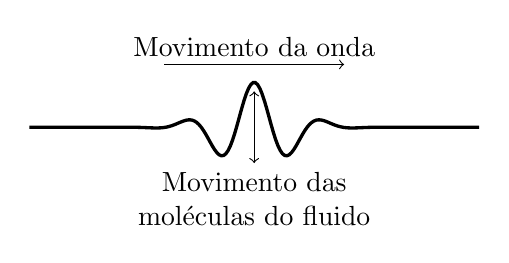
\begin{tikzpicture}
    \begin{axis}[domain=-20:20,ymin=-2,ymax=3, samples=200, axis lines=none]
        \addplot [very thick] {0.5*cos(deg(x))*exp(-x*x/20)};
        \node at (axis cs:0,0.9) {Movimento da onda};
        \draw [->] (axis cs:-8,0.7) -- (axis cs:8,0.7);
        \draw [<->] (axis cs:0,-0.4) -- (axis cs:0,0.4);
        \node [text width=3cm, align=center] at (axis cs:0,-0.8) {Movimento das moléculas do fluido};
    \end{axis}
\end{tikzpicture}

            \caption{Movimento da água na passagem de uma onda
                superficial.\label{fig:oo010}}

        }
    \end{figure}
    Em resultado deste movimento de oscilação vertical da água quando uma onda
    passa, a forma da superfície livre do líquido deixa de ser plana e
    horizontal, notando-se uma perturbação, uma sucessão localizada de pontos da
    superfície acima do nível médio e abaixo do nível médio. De facto, é essa
    perturbação na forma da superfície da água que constitui a onda.

    O que é que se move, então, quando uma onda se propaga na superfície da água
    de lago? É a própria perturbação na forma da superfície da água. 

    Assim, descrever matematicamente as ondas na superfície da água consiste,
    pois, em descrever a perturbação na forma da dessa superfície, e essa
    descrição pode ser feita utilizando uma função que depende do tempo e da
    posição sobre a superfíce, cujo valor é, em cada ponto e em cada instante, o
    do desnível desse ponto relativamente ao nível médio da superfície da água,
    em cada instante.

\item \textbf{Ondas de som}\\
    Quando um som se propaga num gás (por exemplo, em ar), as moléculas desse
    gás adquirem um movimento microscópico de oscilação coletiva (sobreposto ao
    movimento individual de agitação térmica), que se estabelece na direção de
    propagação do som. Por essa razão, no ar ficam definidas regiões de
    compressão e rarefação, que se alternam ao longo da direção da propagação
    (veja a Figura~\ref{fig:oof020}).
    \begin{figure}[htb]
        {\centering
            %\includegraphics{figs/oof020.png}
            \caption{Onda de som e movimento das moléculas de ar.%
                \label{fig:oof020}}

        }
    \end{figure}
    Como no caso das ondas na superfície da água, a \emph{coisa} que aqui se
    propaga ao longo do espaço não é, em rigor, coisa (material) nenhuma, são
    apenas as perturbações nos valores de algumas propriedades do ar (como a
    densidade ou a pressão) relacionadas com as compressões e rarefações
    inerentes à propagação do som. Também aqui devemos introduzir uma função
    (por exemplo, a pressão ou a densidade) cujo valor em cada ponto e em cada
    instante é o da perturbação que constitui a onda de som.

\item \textbf{Ondas numa corda esticada}\\
    Quando se dá um safanão brusco numa corda esticada horizontalmente,
    altera-se a forma da corda. Ela deixa de ser rectilínea\footnote{Na verdade,
    por causa do seu peso, uma corda esticada horizontalmente não assume uma
    forma rigorosamente retilínea, mas antes a forma de uma curva chamada
    \emph{cantenária,} que pode ser apreciada nos cabos de alta tensão, por
    exemplo.}, passando a apresentar uma curva pronunciada induzida pelo
    safanão, que se origina na vizinhança da extremidade agitada e que se
    propaga até à outra.

    De novo, nesta propagação de \emph{algo} ao longo de toda a extensão da
    corda, não ocorre o deslocamento de nenhuma porção de matéria de um dos
    extremos até ao outro. Nenhum segmento de corda se desloca acompanhando a
    propagação. Em vez disso, cada porção de corda apenas realiza algumas
    oscilações, transversais ao sentido da propagação, e de pequena amplitude em
    compa\-ração com a distância percorrida pela \emph{coisa} que se propaga. Na
    verdade, como nos casos anteriores, a entidade que viaja nesta propagação é
    a deformação da corda, a curva nela induzida pelo safanão. Também aqui é
    necessário introduzir uma função para descrever matematicamente a onda,
    função essa que tem, em cada ponto da corda e em cada instante, o valor do
    desvio da corda, nesse ponto, relativamente à sua forma esticada em repouso
    (sem safanões).

\item \textbf{``Ondas'' de espetadores numa bancada de estádio}\\
Nos espetáculos com muitos espetadores é frequente formarem-se ``ondas''
nas bancadas, quando os espetadores numa secção da bancada se levantam
momentaneamente ergendo os braços e sentando-se logo a seguir, sendo
imediatamente imitados pelos que ocupam as secções contíguas, propagando-se esta
ação coletiva até ao extremo da bancada. Nenhum espetador tem que se levantar e
correr ao longo da bancada para que ocorra o movimento da ``onda''; cada
espetador apenas se levanta e se volta a sentar; mas isso é suficiente para que
``algo'' (a onda) viaje ao longo da bancada. Também aqui uma descrição
matemática da ``onda'' parte da introdução de uma função do tempo e do espaço,
função essa cujo valor, em cada ponto e em cada instante, indica se o espetador
com assento nesse ponto estava, nesse instante, levantado ou sentado.
\end{itemize}

\subsection{A função de onda $\psi(x,y,z,t)$}
Nos exemplos de processos ondulatórios que considerámos (e em \emph{todos} os
outros que omitimos), a descrição matemática do fenómeno passa pela introdução
de uma função do tempo e da posição, cujo valor é, em cada instante e em cada
ponto, o da perturbação que constitui a onda em análise. Essa função chama-se
\emph{função de onda} e representa-se normalmente pela letra grega $\psi$ (lê-se
``psi''). A natureza e propriedades gerais desta função (em particular, as
unidades em que é expresso o seu valor) depende da natureza da onda: quando ela
representa um deslocamento (como nas ondulações da superfície dos líquidos ou
nas ondas em cordas), a função de onda tem dimensões de um comprimento e as suas
unidades SI são, portanto, o metro; mas quando, por exemplo, ela representa uma
pressão (como pode ocorrer em ondas de som), então exprime-se, no SI, em pascal.
As ondas eletromagnéticas (e, portanto, a luz) são descritas normalmente pelas
variações do campo eléctrico. Então as unidadas SI da função de onda das ondas
eletromagnéticas são o volt por metro (V/m).

A Figura~\ref{fig:01-020} mostra um impulso ondulatório que se propaga ao longo
do eixo dos $x$, durante um intervalo de tempo $\delta t$. A função de onda está
representada nos dois instantes inicial e final que delimitam esse intervalo.
\begin{figure}[htb]
    {\centering
        \input{sections/01waveintro/figs/f01-020.pgf}\par
    }
    \caption{Impulso ondulatório que se propaga ao longo do eixo dos
    $x$.\label{fig:01-020}}
\end{figure}
No instante inicial $t_1$, a perturbação está localizada numa região próxima da
origem perto da origem; no instante final $t_2$ já se encontra deslocada para a
direita. A função de onda tem representações gráficas diferentes em instantes
diferentes, ou seja: depende do tempo.

Nas condições representadas na Figura~\ref{fig:01-020}, a forma da perturbação
altera-se enquanto ela se propaga. Este comportamento é muito frequente (o som
vai-se alterando com a distância\footnote{O exemplo mais barulhento deste efeito
    nota-se com trovões: o trovão de um relâmpago que ``cai'' perto de nós
    parece um estalo muito intenso, súbito e breve; o de um afastado é aquele
típico ribombar grave e prolongado.}, por exemplo), mas são também frequentes
propagações ondulatórias sem aterações da forma do impulso (por exemplo, na
propagação da luz através do vácuo). As propagações sem alteração de forma são
mais simples e, por isso, é nessas que nos iremos concentrar. Veremos mais à
frente que o formalismo que vai ser desenvolvido pode ainda ser aplicado a
propagações com alteração de forma.

Consideremos então um sinal ondulatório que se propaga com velocidade $v$ ao
longo do eixo dos $x$, sem se alterar a sua forma. Isto significa que a função
matemática que descreve a forma do sinal num dado instante apenas sofre uma
translação por $\delta x=v\delta t$ como resultado da propagação da onda durante
um intervalo de tempo com duração $\delta t$. Assim sendo, podemos escrever
\begin{equation*}
    \psi(x,t) = \psi(x-v(t-t_0),t_0).
\end{equation*}
Escolhendo uma origem temporal adequada $t_0=0$, e notando que não é necessário
explicitar esse instante inicial fixado previamente, concluímos que a função de
onda de um sinal ondulatório que se propaga com velocidade $v$ sem modificação
da forma deve ter a forma geral
\begin{equation*}
    \psi(x,t)=\psi(x-vt).
\end{equation*}

Seja $z=x-vt$. Então $\psi(x-vt)=\psi(z)$ e temos
\begin{align*}
    \pd{\psi}{x}&=\pd{z}{x}\td{\psi}{z}=\td{\psi}{z}&
    \frac{\partial^2\psi}{\partial x^2}&=\pd{z}{x}\td{}{z}\left(\pd{\psi}{x}
        \right)=\frac{\text{d}^2\psi}{\text{d}z^2}\\
    \pd{\psi}{t}&=\pd{z}{t}\td{\psi}{z}=-v\td{\psi}{z}&
    \frac{\partial^2\psi}{\partial t^2}&=\pd{z}{t}\td{}{z}\left(\pd{\psi}{t}
        \right)=v^2\frac{\text{d}^2\psi}{\text{d}z^2}
\end{align*}
Comparando as duas igualdades do lado direito concluímos que
\begin{equation}\label{eq:waveq}
    \frac{\partial^2\psi}{\partial x^2} =
        \frac{1}{v^2} \frac{\partial^2\psi}{\partial t^2}.
\end{equation}
Esta é a equação diferencial satisfeita pelas funções de onda das ondas
unidimensionais que se propagam sem alterações de forma, com velocidade $v$ ao
longo do eixo dos $x$. Chama-se, apropriadamente, \emph{equação de onda
unidimensional.}
Os fenómenos ondulatórios atrás referidos (com a exceção das ondas das bancadas
de estádio), quando reduzidos a uma dimensão, são descritos através funções de
onda que satisfazem a equação de onda unidimensional.



\subsection{O princípio da sobreposição}
Uma vez que a derivada (ou a dupla derivada) de uma combinação linear de funções
é igual a combinação linear correspondente das derivadas de cada
uma\footnote{Isto é,
    $\displaystyle\pd{}{x}(a_1\psi_1+a_2\psi_2+\ldots+a_n\psi_n)=
a_1\pd{\psi_1}{x}+a_2\pd{\psi_2}{x}+\ldots+a_n\pd{\psi_n}{x}.$}, então a soma
de duas soluções (ou a combinação linear de qualquer número de soluções) da
equação de onda é ainda uma solução da equação de onda. A esta propriedade das
ondas chama-se \emph{Princípio da sobreposição.} Em termos práticos, isto
segnifica que quando numa região do espaço coincidem duas ondas com a mesma
natureza $\psi_1(x,y,z,t)$ e $\psi_2(x,y,z,t)$, o valor da perturbação
ondulatória resultante é igual, em cada ponto e em cada instante, à soma das
duas, isto é,
\begin{equation*}
\psi(x,y,z,t)=\psi_1(x,y,z,t)+\psi_2(x,y,z,t).
\end{equation*}

\subsection{Ondas harmónicas}
As funções de onda podem ser (e muito frequentemente são) extraordinariamente
complexas. Mas é possível estabelecer propriedades muito gerais das ondas
considerando apenas funções de onda com forma relativamente simples. De um ponto
de vista matemático, esta possibilidade é afirmada pelo teorema de Fourier,
segundo o qual qualquer função se pode escrever como combinação linear de
funções sinusoidais. É nessas ondas, com forma simples e bem conhecida, que
vamos concentrar o nosso estudo. As propriedades de ondas mais complicadas podem
depois ser deduzidas considerando as sobreposições de ondas sinusoidais que lhes
são equivalentes.

As ondas sinusoidais (que também são conhecidas como \emph{ondas harmónicas} ou
\emph{ondas monocro\-máticas}) são aquelas que têm uma dependência sinusoidal (ou
seja, que são o seno ou o cosseno) da posição e do tempo. Considerando, para
simplificar, apenas ondas unidimensionais (isto é, que dependem de apenas uma
coordenada espacial e do tempo), uma onda sinusoidal é dada pela
expressão geral
\begin{equation*}
    \psi(x,t)=A\cos\left(2\pi\left[\frac{x}{\lambda}\pm \frac{t}{T}\right]+
            \phi_0\right)
\end{equation*}
Nesta equação $x$ e $t$ representam, respetivamente, a posição e o tempo. Os
parâmetros  constantes que aparecem no lado direito têm os nomes
\emph{amplitude} ($A$), \emph{comprimento de onda} ($\lambda$), \emph{período}
($T$) e \emph{constante de fase} ($\phi_0$). Ao valor do argumento do cosseno
dá-se o nome de \emph{fase} da onda harmónica. Os argumentos das funções
transcendentes (como é o caso da função cosseno) devem ser adimensionais; assim,
a fase de uma onda não tem dimensões, pelo que $\lambda$ deve ser um comprimento
e $T$ um tempo. O teor dimensional da amplitude é igual ao da função de onda e
depende, como já vimos, da natureza da onda; frequentemente é um comprimento,
mas pode também ter outras dimensões.

Vejamos o significado e o efeito de cada um destes parâmetros\footnote{O que já
a seguir se segue pode, \emph{e deve,} ser experimentado com uma calculadora
gráfica. Programe a forma da função de onda substituindo os parâmetros por
constantes à sua escolha e dando a $t$ um valor fixo; veja o que acontece no
gráfico quando altera algum dos parâmetros. Para estudar o efeito das variações
no período $T$, deve dar a $x$ um valor determinado e fazer o gráfico de $\psi$
como função do tempo.}.
Na Figura~\ref{fig:01-030} apresentam-se os gráficos de uma função harmónica
como função de $x$, em três instantes $t=0$ (linha contínua), $t=0,15$\,s (linha
a tracejado) e $t=0,3$\,s (linha a ponteado). Na função de onda representada, os
valores dos parâmetros são $A=0,75$, $\lambda=1,5$\,m, $T=1$\,s e $\phi=0$.
Observando o gráfico, notamos que o valor da amplitude, $0,75$, é o módulo dos
extremos de variação da função; notamos também que a distância entre os picos
sucessivos da onda, num determinado instante, tem o valor que atribuímos ao
comprimento de onda $\lambda$.
\begin{figure}[htb]
{\centering
    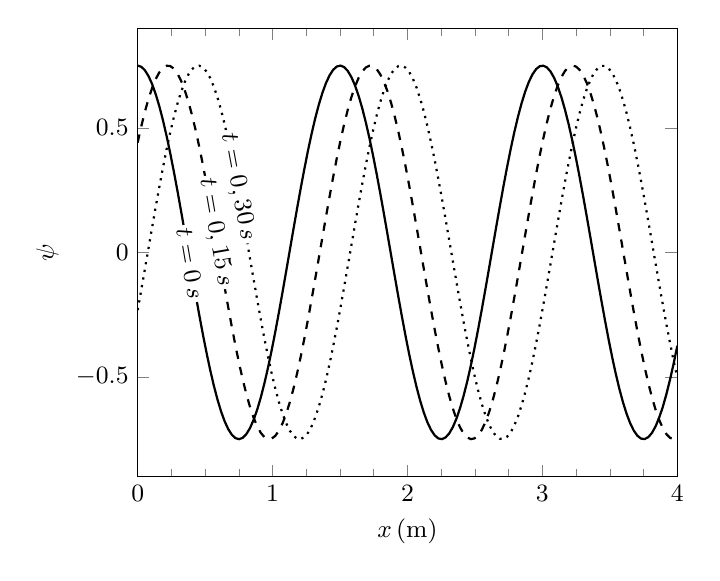
\begin{tikzpicture}
  \small
  \begin{axis}[domain=0:4,
               samples=150,
               xmin=0, xmax=4,
               no marks,
               xlabel=$x$\,(m), ylabel=$\psi$,
               xtick={0,1,2,3,4},
               minor x tick num={3}]
               \addplot [black,thick] {0.75*cos(deg(2*pi*x/1.5))}
            node [ pos=0.1, sloped, fill=white,inner sep=1] {$t=0\,s$};
        \addplot [black, dashed, thick]{0.75*cos(deg(2*pi*(x/1.5-0.15/1.0))}
            node [pos=0.13, sloped, fill=white,inner sep=1] {$t=0,15\,s$};
        \addplot [black, dotted, thick]{0.75*cos(deg(2*pi*(x/1.5-0.30/1.0))}
            node [pos=0.18, sloped, fill=white,inner sep=1] {$t=0,30\,s$};
  \end{axis}
\end{tikzpicture}
\par
}
\caption{Gráficos da função de onda
$\psi(x,t)=A\cos(2\pi[x/\lambda-t/T]+\phi)$, com $A=0,75$, $\lambda=1,5$, $T=1$
e $\phi=0$, para $t=0$ (linha a cheio), $t=0,15$\,s (linha a tracejado) e
$t=0,3$\,s (linha a ponteado).\label{fig:01-030}}
\end{figure}
A figura também mostra que, à medida que o tempo avança, a função de onda
aparece deslocada cada vez mais para a direita: a perturbação sinusoidal
\emph{propaga-se}. Quanto tempo decorre entre a passagem de dois máximos
sucessivos num dado sítio? Da figura, notamos que em 0,3\,s, a onda avança
0,45\,m, ou seja, ela desloca-se com uma velocidade $v = 0,3/0,45=0,6667$\,m/s.
Demorará pois 1\,s a percorrer 1,5\,m, isto é, a distância que separa dois picos
sucessivos. Mas 1\,s é justamente o valor do período $T$. Assim, concluímos o
seguinte:
\begin{itemize}
\item
    a \emph{amplitude} de uma onda harmónica é o valor máximo dos desvios da
    função de onda relativamente ao seu valor médio. É a amplitude da oscilação;
\item
    o \emph{comprimento de onda} de uma onda harmónica é a distância entre
    máximos sucessivos dessa onda;
\item
    o \emph{período} de uma onda harmónica é a duração do intervalo de tempo
    entre a passagem de dois máximos sucessivos da onda num ponto dado.
\end{itemize}
Falta discutir o significado da constante de fase. Este parâmetro está
relacionado com o valor inicial (para $t=0$) da onda na origem (em $x=0$).
Escolhendo, como fizemos acima, $\phi=0$, resulta $\psi(x=0,t=0)=A$. Caso a onda
que queremos descrever se anulasse (por exemplo) no instante inicial e na
origem, escolheríamos $\phi=\pi/2$. Para uma dada onda, podemos sempre escolher
$\phi=0$ definindo de forma conveniente as origens espacial e temporal.
 
A \emph{frequência} de um onda harmónica é o número de máximos da onda que
atingem um determinado ponto por unidade de tempo. Assim, a frequência é o
inverso do período:
\begin{equation*}
    f=\frac{1}{T}.
\end{equation*}
A frequência exprime-se no SI em \emph{ciclos por segundo,} grandeza a que se dá
o nome de \emph{hertz} (Hz).
Outro parâmetro relacionado é a \emph{frequência angular,} que representa também
a rapidez com que a onda varia no tempo, mas agora em radianos por unidade de
tempo:
\begin{equation*}
\omega = 2\pi f= \frac{2\pi}{T}.
\end{equation*}

Podemos calcular facilmente a velocidade de propagação de uma onda harmónica
dividindo o seu comprimento de onda pelo tempo que ela demora a percorrer essa
distância, ou seja, pelo seu período:
\begin{equation*}
v=\frac{\lambda}{T} = \lambda f.
\end{equation*}


\subsection{Intensidade de uma onda harmónica}
As ondas transportam energia. Este facto torna-se óbvio quando consideramos
ondas mecâ\-nicas (ou seja, vibrações coletivas de meios materiais) e constatamos
que é necessária energia para colocar em vibração as várias porções do meio
atingidas pela onda. De onde vem esta energia? Em última análise, essa energia é
fornecida pela fonte e transportada pela onda que a distribui pelos vários
pontos por onde se propaga.

Chama-se \emph{intensidade} de uma onda à energia que ela transporta, por
unidade de tempo e de área. A intensidade de uma onda é sempre proporcional ao
quadrado da sua amplitude, o que se compreende facilmente para o caso das ondas
mecânicas, uma vez que a energia potencial elástica (e são forças elásticas as
responsáveis pela propagação destas ondas) é proporcional ao quadrado da
amplitude do movimento. Mas esta proporcionalidade entre a intensidade de uma
onda e o quadrado da sua amplitude é válida para qualquer tipo de ondas,
incluindo as ondas eletromagnéticas, ou seja, a luz.

\subsection{Sobreposição de ondas harmónicas com iguais comprimento de onda e
período}
\label{sec:sobrpos}
Sejam $\psi_1(x,t)$ e $\psi_2(x,t)$ duas ondas harmónicas com comprimento de
onda $\lambda$ e período $T$, que se propagam no sentido positivo do eixo dos
$x$, dadas por
\begin{align*}
\psi_1(x,t)&=A_1\cos\left(\Theta(x,t)+\phi_1\right)\\
\psi_2(x,t)&=A_2\cos\left(\Theta(x,t)+\phi_2\right),
\end{align*}
onde, para aligeirar a notação, se introduziu o símbolo
$\Theta\equiv\Theta(x,t)=2\pi(x/\lambda-t/T)$. De acordo com o princípio da
sobreposição, a resultante da sobreposição destas duas ondas é uma onda com
expressão geral
\begin{align*}
\psi(x,t)&=\psi_1(x,t)+\psi_2(x,t)\\
&=A_1\cos(\Theta+\phi_1)+A_2\cos(\Theta+\phi_2)
\end{align*}
Usando aqui a igualdade trigonométrica
$\cos(\alpha+\beta)=\cos\alpha\cos\beta-\sin\alpha\sin\beta$, esta expressão
pode reescrever-se como
\begin{equation*}
\psi(x,t)=(A_1\cos\phi_1+A_2\cos\phi_2)\cos\Theta-
(A_1\sin\phi_1+A_2\sin\phi_2)\sin\Theta.
\end{equation*}
Introduzimos agora dois números reais, $A$ e $\phi$, definidos como
\begin{align*}
A\cos\phi&=A_1\cos\phi_1+A_2\cos\phi_2\\
A\sin\phi&=A_1\sin\phi_1+A_2\sin\phi_2.
\end{align*}
Substituindo acima e de novo usando a igualdade trigonométrica para o cosseno da
soma de dois ângulos, obtemos
\begin{equation*}
\psi(x,t)=A\cos\left(\Theta+\phi\right)=
A\cos\left(2\pi\left[\frac{x}{\lambda}-\frac{t}{T}\right]+\phi\right).
\end{equation*}
Assim, concluímos que a sobreposição de duas ondas harmónicas com iguais período
e comprimento de onda é ainda uma onda harmónica, com o mesmo período e com o
mesmo comprimento de onda, com amplitude e constante de fase que dependem das amplitudes
e das constantes de fase de cada uma das ondas que se sobrepõem.

Os números reais $A$ e $\phi$ (a amplitude e a constante de fase da onda
resultante) satisfazem as equações
\begin{align*}
A\cos\phi&=A_1\cos\phi_1+A_2\cos\phi_2\\
A\sin\phi&=A_1\sin\phi_1+A_2\sin\phi_2.
\end{align*}
Elevando estas duas equações ao quadrado, somando os resultados e usando a
igualdade fundamental da trigonometria, obtemos para $A$ a expressão
\begin{equation*}
A^2=A_1^2 + A_2^2 + 2A_1A_2(\cos\phi_1\cos\phi_2+\sin\phi_1\sin\phi_2)
\end{equation*}
Mas a combinação entre parentesis é igual a $\cos(\phi_1-\phi_2)$, que é a
diferença de fase das duas ondas. A amplitude da sobreposição pode então
escrever-se como\footnote{Já agora, é fácil nesta altura demonstrar que a
quantidade real $A$ existe mesmo (até aqui, apenas podíamos garantir que $A^2$
existe. Mas, se acontecer $A^2<0$, então $A$ não pode ser
real.) Com efeito, uma vez que $\cos\delta\phi=\cos(\phi_1-\phi_2)\geq-1$,
segue-se que $A_1^2+A_2^2+2A_1A_2\cos\delta\phi\geq
A_1^2+A_2^2-2A_1A_2=(A_1-A_2)^2\geq 0$. Logo, $A^2\geq0$, ou seja, $A\in
\mathbb{R}$.}
\begin{equation*}
A=\sqrt{A_1^2+A_2^2+2A_1A_2\cos\delta\phi}.
\end{equation*}
%
A constante de fase da onda resultante pode agora também ser facilmente
calculada através de
\begin{align*}
\cos\phi&=\frac{A_1\cos\phi_1+A_2\cos\phi_2}{A}&
\sin\phi&=\frac{A_1\sin\phi_1+A_2\sin\phi_2}{A}.
\end{align*}

\subsection{Interferência construtiva e destrutiva}
\label{sec:condint}
Acabámos de demonstrar que a amplitude da sobreposição de duas ondas harmónicas
com o mesmo comprimento de onda e o mesmo período depende não só das amplitudes
de cada uma, mas também da diferença de fase entre elas. Chamam especial atenção
dois casos particularmente interessantes:
\begin{itemize}
\item \textbf{Interferência construtiva}\\
Quando a diferença entre as fases das duas ondas é um múltiplo inteiro de $2\pi$,
isto é, quando
\begin{equation*}
\delta\phi = 2k\pi,\quad k=0,\pm1,\pm2,\ldots,
\end{equation*}
o seu cosseno vale um, e assim a amplitude da sobreposição resulta
\begin{equation*}
A=\sqrt{A_1^2 + A_2^2+2A_1A_2}=\sqrt{(A_1+A_2)^2}=A_1+A_2.
\end{equation*}
Ou seja, quando a diferença de fase é um múltiplo inteiro de $2\pi$ a amplitude
da sobre\-posição é igual à soma das amplitudes das duas ondas que se sobrepõem;
as duas ondas reforçam-se mutuamente resultando uma onda de amplitude maior do
que a de qualquer das duas. Dizemos nestas condições que as duas ondas estão
\emph{em fase} e que \emph{interferem construtivamente.}
\item \textbf{Interferência destrutiva}\\
Quando a diferença entre as fases das duas ondas é um múltiplo semi-inteiro de
$2\pi$, ou seja, quando
\begin{equation*}
\delta\phi = 2\left(k+\frac{1}{2}\right)\pi,\quad k=0,\pm1,\pm2,\ldots,
\end{equation*}
então o seu cosseno vale agora $-1$ e obtemos para a amplitude da sobreposição
\begin{equation*}
A=\sqrt{A_1^2 + A_2^2 - 2A_1A_2} = \sqrt{(A_1-A_2)^2}=\left|A_1-A_2\right|.
\end{equation*}
Agora, verifica-se que a amplitude da sobreposição das duas ondas é menor do que
a maior das duas; as duas ondas interferem atenuando-se. Dizemos agora que as
duas ondas se encontram em \emph{oposição de fase} e que \emph{interferem
destrutivamente.}
\end{itemize}
Note-se que a atenuação que ocorre quando há interferência destrutiva pode ser
total. Se as amplitudes das duas ondas que interferem forem iguais, e se elas
estiverem em oposição de fase, então a amplitude resultante é nula: a onda
resultante não existe.

Vimos que o valor da constante de fase de uma onda é, no essencial, fixado
por nós arbitrariamente, já que depende da escolha que fazemos para a posição da
origem do sistema de coordenadas e para o isntante que consideramos inicial.
Nessa medida, a constante de fase parece não ter um significado físico muito
relevante. É verdade, mas o mesmo não se pode dizer da \emph{diferença de fase}
de duas ondas (e, se elas tiverem o mesmo comprimento de onda e a mesma
frequência, essa diferença é igual à diferença entre as suas constantes de
fase). O resultado da sobreposição de duas ondas depende dramaticamente da
diferença entre as suas fases. Ou seja, a diferença entre as duas irrelevâncias
é muitíssimo relevante.

\subsection{Diferença entre as fases de uma onda em dois pontos do seu trajeto}
\label{sec:dfidx}
Uma vez que a diferença de fase desempenha um papel tão importante nos fenómenos
de interferência, é importante saber calculá-la em diferentes situações.
Frequentemente, a diferença de fase entre as duas ondas resulta de terem
percorrido caminhos com comprimento diferente e, assim, é importante saber
calcular a variação na fase de uma onda de um ponto para outro. 
Sejam $x_1$ e $x_2$ as coordenadas de dois pontos no eixo dos $x$ e consideremos
uma onda harmónica genérica que se propaga segundo esse eixo, dada por
\begin{equation*}
\psi(x,t)=A\
    cos\left(2\pi\left[\frac{x}{\lambda}-\frac{t}{T}\right]+\phi\right).
\end{equation*}
A fase que esta onda apresenta nos dois pontos num dado instante é
\begin{align*}
\phi_1&=2\pi\left(\frac{x_1}{\lambda}-\frac{t}{T}\right)+\phi\\
\phi_2&=2\pi\left(\frac{x_2}{\lambda}-\frac{t}{T}\right)+\phi.
\end{align*}
A variação de fase é, então,
\begin{equation*}
\delta\phi=\phi_2-\phi_1=2\pi\frac{x_2-x_1}{\lambda}.
\end{equation*}

\subsection{Frentes de onda}
Até agora, sempre que foi necessário entrar em detalhes matemáticos,
considerámos ondas unidimensionais, ou seja, ondas cuja função só depende de uma
coordenada espacial e do tempo. No essencial, isso será suficiente neste estudo,
mas, em grande medida para introduzir alguns termos de uso corrente, devemos
agora analisar as ondas no espaço tridimensional.

Os pontos do espaço onde a função de onda tem a mesma fase definem linhas (para
ondas definidas num espaço bidimensional, como as ondas do mar, ou as vibrações
da pele de um tambor) ou superfícies, para as ondas definidas no espaço usual do
dia a dia (que tem três dimensões). Essas regiões do espaço onde a fase de uma
onda tem o mesmo valor chamam-se \emph{frentes de onda}\footnote{Na praia,
chamamos \emph{onda} às frentes de onda para as quais a função de onda tem um
máximo. São também frentes de onda os intervalos entre as ``ondas'', aquelas
regiões onde o ``vale'' da onlulação atinge a sua profundidade máxima.}. As
frentes de onda das ondas que se formam na superfície de um lago calmo quando
nela cai uma pedra têm forma circular, com centro no ponto da superfície onde a
pedra caiu; as das ondas de choque de uma explosão aérea têm forma esférica, com
centro no ponto onde a explosão se deu; as das ondas de som produzidas por uma
fonte sonora muito afastada são também esféricas, mas o seu raio é tão elevado
que, para muitos efeitos, é como se fossem planas (tal como a superfície da
Terra: é esférica mas, quase sempre, pensamos nela como plana). A
Figura~\ref{fig:oof040} ilustra algumas frentes de onda de uma onda plana.
\begin{figure}[htb]
{\centering
%\includegraphics{figs/oof040.png}
\caption{Diferentes frentes de onda (ou a mesma frente, representada em
instantes diferentes) de uma onda plana que se propaga na direção do eixo dos
$x$.\label{fig:oof040}}

}
\end{figure}
Note-se que cada porção da frente de onda propaga-se na direcção que lhe é
perpendicular. Assim, a Figura~\ref{fig:oof040} pode também interpretar-se como
uma representação da \emph{mesma} frente de onda, em diferentes instantes.

\subsection{Princípio de Huygens}
Na propagação de uma onda, a causa directa para que a perturbação ondulatória se
manifeste num dado ponto é que ela se tenha manifestado nos pontos vizinhos. Por
outras palavras, a fonte da perturbação ondulatória num dado local é a própria
perturbação na vizinhança desse local. Esta constatação inspirou o chamado
\emph{princípio de Huygens}:
\begin{quote}
    \textsl{Cada ponto numa frente de onda é fonte de ondas secundárias cuja
    interferência mútua determina a forma da frente de onda em instantes
    posteriores.}
\end{quote}
Usando este princípio é possível demonstrar as leis da ótica geométrica e ainda
compreender os fenómenos em que a natureza ondulatória da luz se manifesta e que
constituem o assunto deste capítulo.


\subsection{Ondas --- Resumo}
\begin{itemize}
\item
    Função de onda de ondas harmónicas unidimensionais:
    \begin{equation*}
    \psi(x,t)=A\cos\left(2\pi\left[\frac{x}{\lambda}\pm\frac{t}{T}\right]+
                \phi\right),
    \end{equation*}
    com
    \begin{center}
    \begin{tabular}{c|l|l|l}
    \hline
    \rule{0mm}{3ex} Símbolo&Nome&Dimensões&Significado\\[0.5ex]
    \hline
    $A$ & Amplitude & Depende&
        \parbox[t]{0.3\textwidth}{\rule{0mm}{4ex}Módulo dos desvios máxi\-mos
        relativamente ao valor médio}\\
    $\lambda$ & Comprimento de onda & Comprimento &
        \parbox[t]{0.3\textwidth}{\rule{0mm}{4ex}Distância entre máximos da função
        de onda sucessivos} \\
    $T$ & Período & Tempo &
        \parbox[t]{0.3\textwidth}{\rule{0mm}{4ex}Intervalo de tempo entre a
        passagem, num ponto fixo, de dois máximos da função de onda sucessivos}
    \\
    $\phi$&Constante de fase&Adimensional&
        \parbox[t]{0.3\textwidth}{\rule{0mm}{4ex}Fase da função de onda na
        origem do sistema de coordenadas, no instante $t=0$}\\[5ex]
    \hline
    \end{tabular}
    \end{center}
\item Frequência de uma onda harmónica: \\
Frequência: $f=1/T$. Unidades: ciclos por segundo ou Hz (hertz).\\
Frequância angular: $\omega = 2\pi f=2\pi/T$. Unidades: rad/s ou s$^{-1}$
\item Velocidade de propagação de uma onda harmónica:
\begin{equation*}
v=\frac{\lambda}{T}=\lambda f=\lambda \omega/2\pi
\end{equation*}
\item Condições especiais de interferência: \\
Interferência construtiva: $\delta\phi=2k\pi,\quad k=0,\pm1,\pm2,\ldots$\\
Interferência destrutiva: $\delta\phi=2(k+1/2)\pi,\quad k=0,\pm1,\pm2,\ldots$

\item Diferença entre as fases de uma onda harmónica em dois pontos do seu
trajeto a uma distância $d$ um do outro:
\begin{equation*}
\delta \phi = 2\pi\frac{d}{\lambda}.
\end{equation*}
\item Intensidade de uma onda: energia transportada pela onda por unidade de
    tempo e de área (densidade do fluxo de potência). É sempre proporcional ao
    quadrado da sua amplitude:
    \begin{equation*}
        I\alpha A^2
    \end{equation*}
\end{itemize}

